\section{任务二}
\subsection{任务内容}
实现多进程同时访问文件、目录功能。
\subsection{任务实现规划}
该问题即是实现读者写者问题,其中读者进程可以同时访问文件和目录,写者进程必须与读者进程和其他写者进程互斥地访问文件(即写者创建、删除文件和目录必须是互斥的)。
由于真正的fork()需要共享内存,信号量需要在父子进程间通信,实现起来过于复杂,因此采用pthread线程模拟进程(线程可以自然共享全局变量)。实现进程同步时采用经典读者写者问题的解决方法,其中需要互斥的操作如
创建和删除文件、目录;写文件和读文件等需要信号量控制互斥地打开,因此涉及这些操作的函数必须加锁。

\subsubsection{头文件常量定义与函数声明}
在include文件夹中的fat.h文件中需要修改原来的DirEntry结构体,加上属于该文件的读写锁rwlock;定义全局互斥锁用于保护修改读者数量的信号量fs\_mutex;
定义进程控制块结构体PCB,用以维护当前进程信息。具体代码如下:
\begin{ccode}{fat.h}
/*系统是基于内存的：建立一个数组,把这个数组当成硬盘,实现文件系统。
假设只有一个进程使用。*/
#include <stdio.h>
#include <string.h>
#include <stdlib.h>
#include <stdbool.h>
#include <pthread.h>
#include <semaphore.h>

//定义所用常量
#define DISK_MAXLEN 2560
#define BLOCK_SIZE 64
#define BLOCK_NUM (DISK_MAXLEN / BLOCK_SIZE)
#define MAX_ENTRY 32
#define MAX_OPEN_FILE 32
#define MAX_FD 16

//最大进程数
#define MAX_PROCESS 8

//模式定义
#define MODE_READ  1
#define MODE_WRITE 2
#define MODE_RDWR  3
#define MODE_WAPPEND 4

//目录项
typedef struct {
    char name[16];
    int size;
    int start_block;
    int ac;
    int type;
    int parent;
    int reader_count;           /* 当前读者数量 */
    sem_t rw_lock;              /* 文件资源信号量,初值=1 */
    pthread_mutex_t mutex;      /* 保护 reader_count 的互斥锁 */
} DirEntry;

//文件描述符
typedef struct {
    int used;       // 0 空闲,1 已使用
    int dir_index;  // 对应 Directory[] 下标
    int offset;     // 当前读写偏移
    int mode;       // 打开模式
} FileDescriptor;

//pcb
typedef struct {
    int pid;
    FileDescriptor fd_table[MAX_FD];
    int current_dir;          // 每个进程维护的当前目录索引
} PCB;


extern char Disk[DISK_MAXLEN];
extern int FAT[BLOCK_NUM];
extern DirEntry Directory[MAX_ENTRY];
extern pthread_mutex_t fs_mutex;
extern PCB ProcessTable[MAX_PROCESS];


void init_fs(void);
void init_process_table(void);

//目录操作
bool mkdir(int pid, const char *dirname);
bool ls(int pid);
bool cd(int pid, const char *dirname);

//文件创建与删除
bool fs_create(int pid, const char *filename);
bool fs_delete(const char *filename);

//文件打开关闭与读写
int  fs_open(int pid, const char *filename, int mode);
bool fs_close(int pid, int fd);
int  fs_read(int pid, int fd, char *buffer, int size);
int  fs_write(int pid, int fd, const char *data, int size);
bool fs_seek(int pid, int fd, int offset);


void print_prompt(int pid);

\end{ccode}
其中相较于任务一的主要修改为:改为每个进程单独维护当前目录索引current\_dir,而不是全局维护一个;所有目录、文件操作函数都需要添加pid参数用以指定当前进程;
目录项结构体DirEntry中新增reader\_count字段用以维护当前读者数量,rw\_lock信号量用于保护文件资源,mutex互斥锁用来保护对reader\_count的修改。
\input{content/task2/052system_init}
\subsubsection{文件目录操作}
在src文件夹中的dir.c文件中实现多进程下访问目录功能,这里显然创建目录、列出当前目录下所有文件及文件夹操作都需要互斥进行,具体代码如下:
\begin{ccode}{目录操作函数}
#include "fat.h"

bool mkdir(int pid, const char *dirname)
{
    if (pid < 0 || pid >= MAX_PROCESS) return false;
    int cur_dir = ProcessTable[pid].current_dir;

    pthread_mutex_lock(&fs_mutex);//创建文件需要加锁

    for (int i = 0; i < MAX_ENTRY; i++) {
        if (Directory[i].ac == 0) {
            strncpy(Directory[i].name, dirname, 16);
            Directory[i].size = 0;
            Directory[i].start_block = -1;
            Directory[i].ac = 1;
            Directory[i].type = 1;
            Directory[i].parent = cur_dir;
            Directory[i].reader_count = 0;
            sem_init(&Directory[i].rw_lock, 0, 1);
            pthread_mutex_init(&Directory[i].mutex, NULL);
            pthread_mutex_unlock(&fs_mutex);
            return true;
        }
    }

    pthread_mutex_unlock(&fs_mutex);
    return false;
}

static int get_dir_size(int dir_index)
{
    int total = 0;
    for (int i = 0; i < MAX_ENTRY; i++) {
        if (Directory[i].ac == 1 && Directory[i].parent == dir_index) {
            if (Directory[i].type == 0) {
                total += Directory[i].size;
            } else if (Directory[i].type == 1) {
                total += get_dir_size(i);
            }
        }
    }
    return total;
}

bool ls(int pid)
{
    if (pid < 0 || pid >= MAX_PROCESS) return false;
    int cur_dir = ProcessTable[pid].current_dir;

    pthread_mutex_lock(&fs_mutex);

    for (int i = 0; i < MAX_ENTRY; i++) {
        if (Directory[i].ac == 1 && Directory[i].parent == cur_dir) {
            int show_size;
            if (Directory[i].type == 1) {
                show_size = get_dir_size(i);
            } else {
                show_size = Directory[i].size;
            }
            printf("%s\t%s\t%d bytes\n",
                   Directory[i].type == 1 ? "DIR" : "FILE",
                   Directory[i].name,
                   show_size);
        }
    }

    pthread_mutex_unlock(&fs_mutex);
    return true;
}

bool cd(int pid, const char *dirname)
{
    if (pid < 0 || pid >= MAX_PROCESS || dirname == NULL) return false;

    int cur_dir = ProcessTable[pid].current_dir;

    if (strcmp(dirname, "/") == 0) {
        ProcessTable[pid].current_dir = 0;
        return true;
    }

    if (strcmp(dirname, "..") == 0) {
        if (Directory[cur_dir].parent != -1) {
            ProcessTable[pid].current_dir = Directory[cur_dir].parent;
        }
        return true;
    }

    //遍历以在当前目录下找子目录(对Directory[]只读),避免其他进程此时mkdir/touch,加锁保证一致性
    pthread_mutex_lock(&fs_mutex);

    for (int i = 0; i < MAX_ENTRY; i++) {
        if (Directory[i].ac == 1 &&
            Directory[i].parent == cur_dir &&
            Directory[i].type == 1 &&
            strcmp(Directory[i].name, dirname) == 0) {
            ProcessTable[pid].current_dir = i;
            pthread_mutex_unlock(&fs_mutex);
            return true;
        }
    }

    pthread_mutex_unlock(&fs_mutex);
    return false;
}
\end{ccode}
目录操作有关函数首先需要提取进程控制块中存放的当前目录位置作为实际工作目录。mkdir()函数在查找空闲目录项前需要申请信号量(pthread\_mutex\_lock(\&fs\_mutex)),查找完成后成功
获取空闲Directory项作为新建目录项或查找失败,都需要释放信号量(pthread\_mutex\_unlock(\&fs\_mutex)),其中成功获取空闲项并修改的操作与任务一相同。类似地,ls()函数和cd()函数的核心操作与任务一中类似,
只是在需要互斥访问目录项数组Directory时需要前后加信号量保护。
\subsubsection{文件打开与关闭}
在src文件夹的file.c文件中实现对文件的打开与关闭操作,由于这里每个进程实际都有可能是写者和读者,因此打开文件时不区分是读进程还是写进程,只根据打开文件的模式来判断,具体代码如下:
\begin{itemize}
    \item 打开文件
    \begin{ccode}{打开文件函数}
int fs_open(int pid, const char *filename, int mode)
{
    if (pid < 0 || pid >= MAX_PROCESS || filename == NULL) {
        return -1;
    }

    int cur_dir = ProcessTable[pid].current_dir;
    int dir_index = -1;

    //互斥访问Directory,查找要打开的文件
    pthread_mutex_lock(&fs_mutex);

    for (int i = 0; i < MAX_ENTRY; i++) {
        if (Directory[i].ac == 1 &&
            Directory[i].parent == cur_dir &&
            Directory[i].type == 0 &&
            strcmp(Directory[i].name, filename) == 0) {
            dir_index = i;
            break;
        }
    }

    if (dir_index == -1) {
        pthread_mutex_unlock(&fs_mutex);
        printf("open failed: file not found: %s\n", filename);
        return -1;
    }

    pthread_mutex_unlock(&fs_mutex);

    //只读、读写打开文件需要修改reader_count数量(互斥修改)

    if (mode == MODE_READ) {
        pthread_mutex_lock(&Directory[dir_index].mutex);//互斥修改reader_count
        Directory[dir_index].reader_count++;
        if (Directory[dir_index].reader_count == 1) {
            if (sem_trywait(&Directory[dir_index].rw_lock) != 0) { //有写者时打开失败
                Directory[dir_index].reader_count--;
                pthread_mutex_unlock(&Directory[dir_index].mutex);
                printf("open failed: file is busy\n");
                return -1;
            }
        }
        pthread_mutex_unlock(&Directory[dir_index].mutex);//修改reader_count结束
    }
    else if (mode == MODE_WRITE || mode == MODE_RDWR) {
        if (sem_trywait(&Directory[dir_index].rw_lock) != 0) {  //文件被读者或写者占用时访问失败
            printf("open failed: file is busy\n");
            return -1;
        }
    }
    else {
        printf("open failed: invalid mode\n");
        return -1;
    }

    //分配fd
    for (int fd = 0; fd < MAX_FD; fd++) {
        if (ProcessTable[pid].fd_table[fd].used == 0) {
            ProcessTable[pid].fd_table[fd].used = 1;
            ProcessTable[pid].fd_table[fd].dir_index = dir_index;
            ProcessTable[pid].fd_table[fd].offset = 0;
            ProcessTable[pid].fd_table[fd].mode = mode;

            printf("open success: pid=%d, file=%s, fd=%d\n",
                   pid, filename, fd);
            return fd;
        }
    }

    //fd分配失败,回退已经做的修改
    if (mode == MODE_READ) {
        pthread_mutex_lock(&Directory[dir_index].mutex);
        Directory[dir_index].reader_count--;
        if (Directory[dir_index].reader_count == 0) {
            sem_post(&Directory[dir_index].rw_lock);  // 最后一个读者释放文件 
        }
        pthread_mutex_unlock(&Directory[dir_index].mutex);
    } else {
        sem_post(&Directory[dir_index].rw_lock);  // 写者释放文件 
    }

    printf("open failed: fd table full\n");
    return -1;
}
    \end{ccode}
    整体实现思路类似任务一,在Directory数组中查找要打开的文件时前后加锁保护,确保一致性。之后按读者-写者问题的经典解法实现:
    当以只读模式(MODE\_READ)打开时,该进程视为读者,需要先互斥修改reader\_count(通过pthread\_mutex\_lock/unlock对mutex加锁/解锁),若为第一个读者,还需对资源信号量执行P操作(sem\_trywait(\&Directory[dir\_index].rw\_lock)),以阻塞后续写者;
    当以只写模式(MODE\_WRITE)或读写模式(MODE\_RDWR)打开时,该进程视为写者,直接对资源信号量执行P操作,确保对文件的互斥访问,阻止其他读者和写者。
    这里实现时使用\texttt{sem\_trywait}而非\texttt{sem\_wait},原因是若使用sem\_wait阻塞等待,当前交互界面会被卡住,无法手动切换进程并释放资源。因此本实验采用非阻塞方式,即文件被占用时直接返回失败。在实际多进程环境中应当使用真正的阻塞等待来实现互斥。
    对于打开的文件需要分配文件描述符fd,当fd表已满时意味着文件打开失败,此时需要回退前一步做的修改,即恢复reader\_count以及释放资源信号量(sem\_post)。
    \item 关闭文件
    \begin{ccode}{关闭文件函数}
bool fs_close(int pid, int fd)
{
    if (pid < 0 || pid >= MAX_PROCESS || fd < 0 || fd >= MAX_FD) {
        return false;
    }

    if (ProcessTable[pid].fd_table[fd].used == 0) {
        printf("close failed: invalid fd\n");
        return false;
    }

    int dir_index = ProcessTable[pid].fd_table[fd].dir_index;
    int mode = ProcessTable[pid].fd_table[fd].mode;


    if (mode == MODE_READ) {
        pthread_mutex_lock(&Directory[dir_index].mutex);
        Directory[dir_index].reader_count--;
        if (Directory[dir_index].reader_count == 0) {
            sem_post(&Directory[dir_index].rw_lock);  // 最后一个读者释放文件 
        }
        pthread_mutex_unlock(&Directory[dir_index].mutex);
    }
    else if (mode == MODE_WRITE || mode == MODE_RDWR) {
        sem_post(&Directory[dir_index].rw_lock);  // 写者释放文件 
    }
    
    //释放已分配的fd
    ProcessTable[pid].fd_table[fd].used = 0;
    ProcessTable[pid].fd_table[fd].dir_index = -1;
    ProcessTable[pid].fd_table[fd].offset = 0;
    ProcessTable[pid].fd_table[fd].mode = 0;

    printf("close success: pid=%d, fd=%d\n", pid, fd);
    return true;
}
    \end{ccode}
     同样采用读者-写者问题的经典解法,类似打开文件的实现。根据进程数组中对应文件描述符记录的打开模式确定是读者还是写者:
     写者(MODE\_WRITE或MODE\_RDWR)直接释放资源信号量即可;读者(MODE\_READ)需要先互斥减少reader\_count,当reader\_count降为0时由最后一个读者释放资源信号量。
\end{itemize}

\subsection{任务二函数汇总}
下表对任务二实现的所有主要函数进行汇总,以便对照查阅。

\begin{table}[H]
\centering
\caption{任务二主要函数汇总}
\label{tab:task2_summary}
\resizebox{\textwidth}{!}{%
\begin{tabular}{|c|c|c|c|c|}
\hline
\textbf{函数名} & \textbf{功能} & \textbf{实现方法} & \textbf{关键数据结构} & \textbf{同步机制} \\
\hline
\texttt{init\_fs()} & 初始化文件系统 & 新增信号量/互斥锁初始化,调用init\_process\_table() & Directory[].rw\_lock, .mutex & 信号量初值置1,互斥锁初始化 \\
\hline
\texttt{init\_process\_table()} & 初始化PCB数组 & memset清零,设置pid和current\_dir & ProcessTable[] & 无 \\
\hline
\texttt{mkdir(pid,...)} & 创建目录 & 互斥锁保护Directory数组,查找空闲项设置属性 & Directory[], fs\_mutex & 互斥锁保护全局目录项 \\
\hline
\texttt{ls(pid,...)} & 列出当前目录内容 & 互斥锁保护下遍历Directory并打印 & Directory[], fs\_mutex & 互斥锁保护读取一致性 \\
\hline
\texttt{cd(pid,...)} & 切换当前目录 & 互斥锁保护下查找目标目录,更新进程current\_dir & Directory[], ProcessTable[] & 互斥锁防止mkdir干扰 \\
\hline
\texttt{fs\_create(pid,...)} & 创建文件 & 互斥锁保护Directory,找空闲项设置属性 & Directory[], fs\_mutex & 互斥锁 \\
\hline
\texttt{fs\_delete()} & 删除文件 & 遍历Directory找文件,沿FAT链释放块 & Directory[], FAT[], fs\_mutex & 互斥锁 \\
\hline
\texttt{fs\_open(pid,...)} & 打开文件 & 互斥锁查找文件→读者:加reader\_count,首读者P(rw\_lock);写者:直接P(rw\_lock)→分配fd & Directory[].rw\_lock, .mutex & 读者-写者经典解法,sem\_trywait非阻塞 \\
\hline
\texttt{fs\_close(pid,...)} & 关闭文件 & 读者:减reader\_count,末读者V(rw\_lock);写者:V(rw\_lock)→清零fd表项 & Directory[].rw\_lock, .mutex & 读者-写者释放逻辑 \\
\hline
\texttt{fs\_read(pid,...)} & 读取文件内容 & 沿FAT链从offset逐块读取到buffer & Disk[], FAT[], ProcessTable[] & 依赖open时的rw\_lock保护 \\
\hline
\texttt{fs\_write(pid,...)} & 写入文件内容 & 确保FAT链有足够块,从offset逐块写入 & Disk[], FAT[], ProcessTable[] & 依赖open时的rw\_lock保护 \\
\hline
\end{tabular}%
}
\end{table}

\subsubsection{文件读写}
在src文件夹中的file.c文件中实现文件的读写、删除等函数,其实方法类似任务一,只是在查找目录项、FAT表时为了确保互斥访问和一致性,需要前后申请信号量保护。
重点修改在删除文件时需要确保没有读者或写者在使用该文件,否则无法删除,具体代码如下:
\begin{ccode}{删除文件函数}
bool fs_delete(const char *filename)
{
    pthread_mutex_lock(&fs_mutex);

    for (int i = 0; i < MAX_ENTRY; i++) {
        if (Directory[i].ac == 1 &&
            Directory[i].type == 0 &&
            strcmp(Directory[i].name, filename) == 0) {

            // 检查文件是否正被打开：
            //  reader_count > 0 说明有读者
            //  sem_trywait(&rw_lock) 失败说明有写者
            pthread_mutex_lock(&Directory[i].mutex);
            if (Directory[i].reader_count > 0) {
                pthread_mutex_unlock(&Directory[i].mutex);
                pthread_mutex_unlock(&fs_mutex);
                printf("Failed to delete file: %s is in use\n", filename);
                return false;
            }
            pthread_mutex_unlock(&Directory[i].mutex);

            if (sem_trywait(&Directory[i].rw_lock) != 0) {
                pthread_mutex_unlock(&fs_mutex);
                printf("Failed to delete file: %s is in use\n", filename);
                return false;
            }
            sem_post(&Directory[i].rw_lock);  // 成功拿到写锁，立即释放 

            int cur = Directory[i].start_block;
            while (cur != -1) {
                int next = FAT[cur];
                FAT[cur] = 0;
                if (next == -1) break;
                cur = next;
            }

            Directory[i].ac = 0;
            pthread_mutex_unlock(&fs_mutex);
            printf("File deleted successfully: %s\n", filename);
            return true;
        }
    }

    pthread_mutex_unlock(&fs_mutex);
    printf("Failed to delete file: %s\n", filename);
    return false;
}
\end{ccode}
如果检查到reader\_count大于0,说明还有读者在访问文件,无法删除;如果检查到sem\_trywait(\&rw\_lock)返回失败,说明有写者在访问文件,同样无法删除。只有当文件空闲没有进程在访问时,才能删除文件,具体删除操作于任务一相同,释放占有的FAT表项和Directory目录项即可。
\subsubsection{文件系统入口}
在src文件夹的main.c文件中实现文件系统入口函数,实现同样类似任务一,不同点在于需要实现进程的切换,这里通过维护当前进程号pid的全局变量current\_pid实现。
具体代码如下:
\begin{ccode}{进程切换}
//切换当前操作的进程 
        else if (strcmp(cmd, "pid") == 0) {
            int new_pid;
            if (sscanf(line, "%31s %d", cmd, &new_pid) == 2) {
                if (new_pid >= 0 && new_pid < MAX_PROCESS) {
                    current_pid = new_pid;
                    printf("switched to pid %d\n", current_pid);
                } else {
                    printf("invalid pid (0-%d)\n", MAX_PROCESS - 1);
                }
            } else {
                printf("usage: pid <0-%d>\n", MAX_PROCESS - 1);
            }
        }
\end{ccode}
这里当接收到用户pid n的命令时会尝试将current\_pid切换为n(n在0到MAX\_PROCESS-1之间视为合法进程号),此后的操作会基于新的进程进行。其他操作如mkdir、open等命令格式与任务一相同,虽然在函数声明时需要传入
pid参数,但这里会自动传入current\_pid,无需手动传递。
\subsubsection{多进程访问测试}
上述代码修改完成后即可实现多进程同时访问文件、目录的功能,代码编译运行结果如下图所示:
\begin{figure}[H]
    \centering
    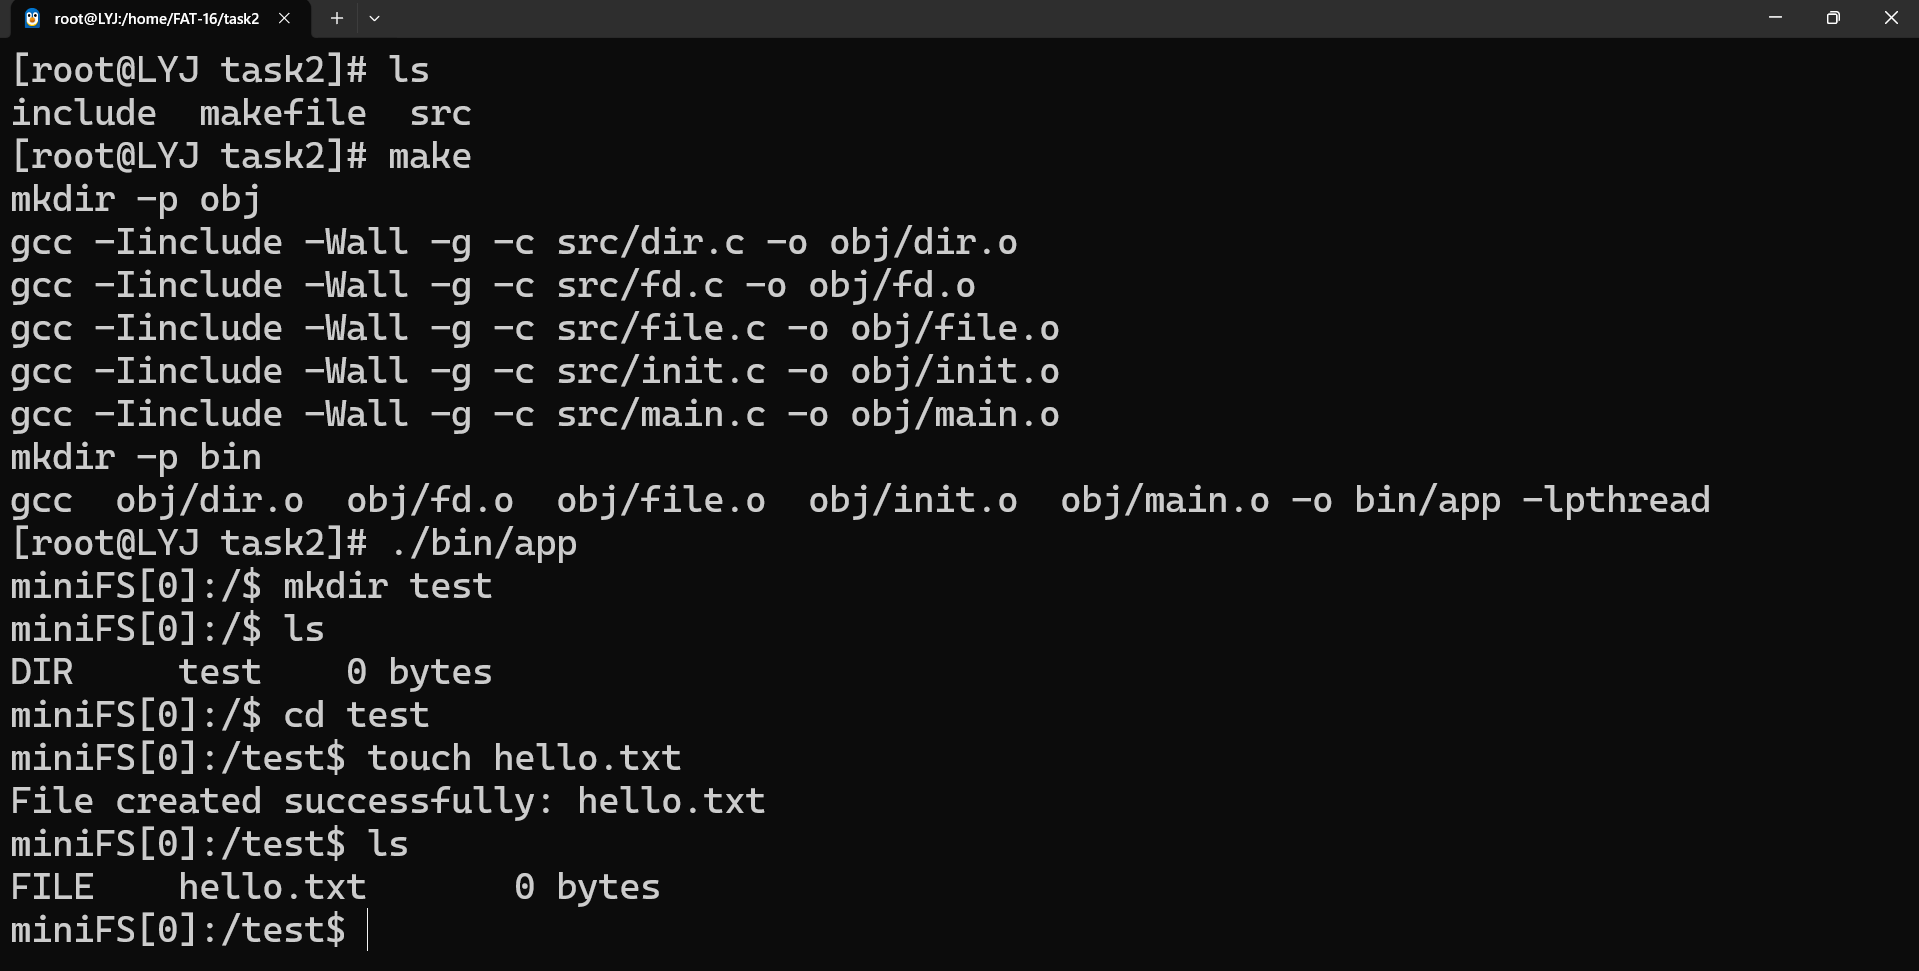
\includegraphics[width=1\textwidth]{figure/task2_common_function.png}
    \caption{文件系统一般操作}
\end{figure}
如上图所示,一般的创建文件夹、创建文件以及切换目录等操作能够正常实现。

\begin{figure}[H]
    \centering
    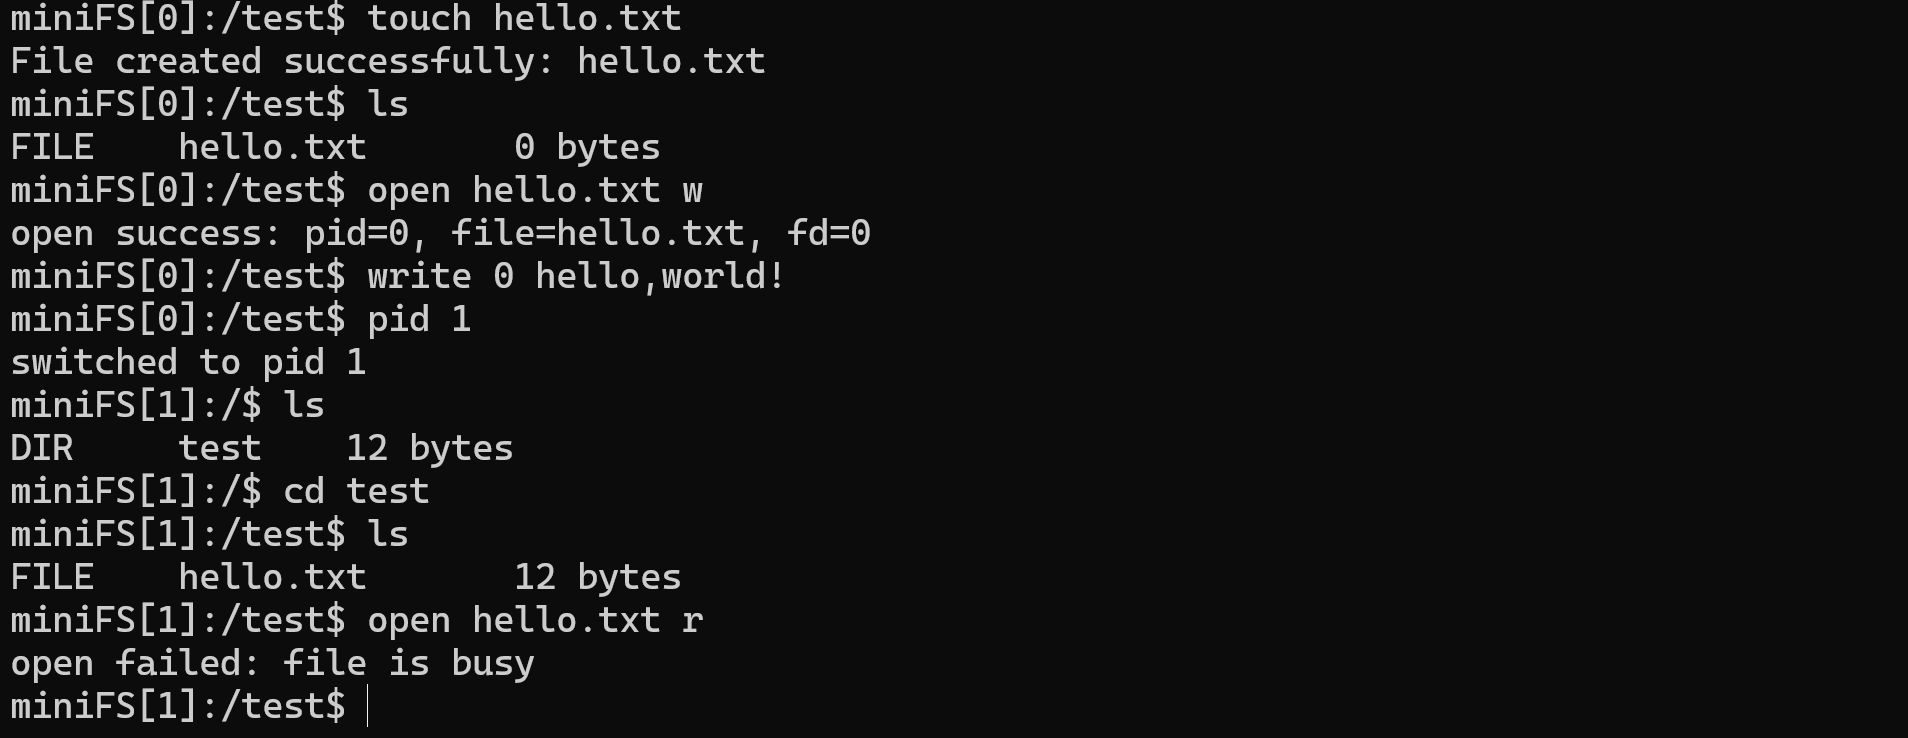
\includegraphics[width = 1\textwidth]{figure/task2_writeonly.png}
    \caption{写进程与读进程互斥}
\end{figure}
如上图所示,当一个写进程(pid=0)打开文件时,切换其他读进程(pid=1)尝试打开文件失败,提示"file is busy",说明能实现写进程互斥访问文件的功能。

\begin{figure}[H]
    \centering
    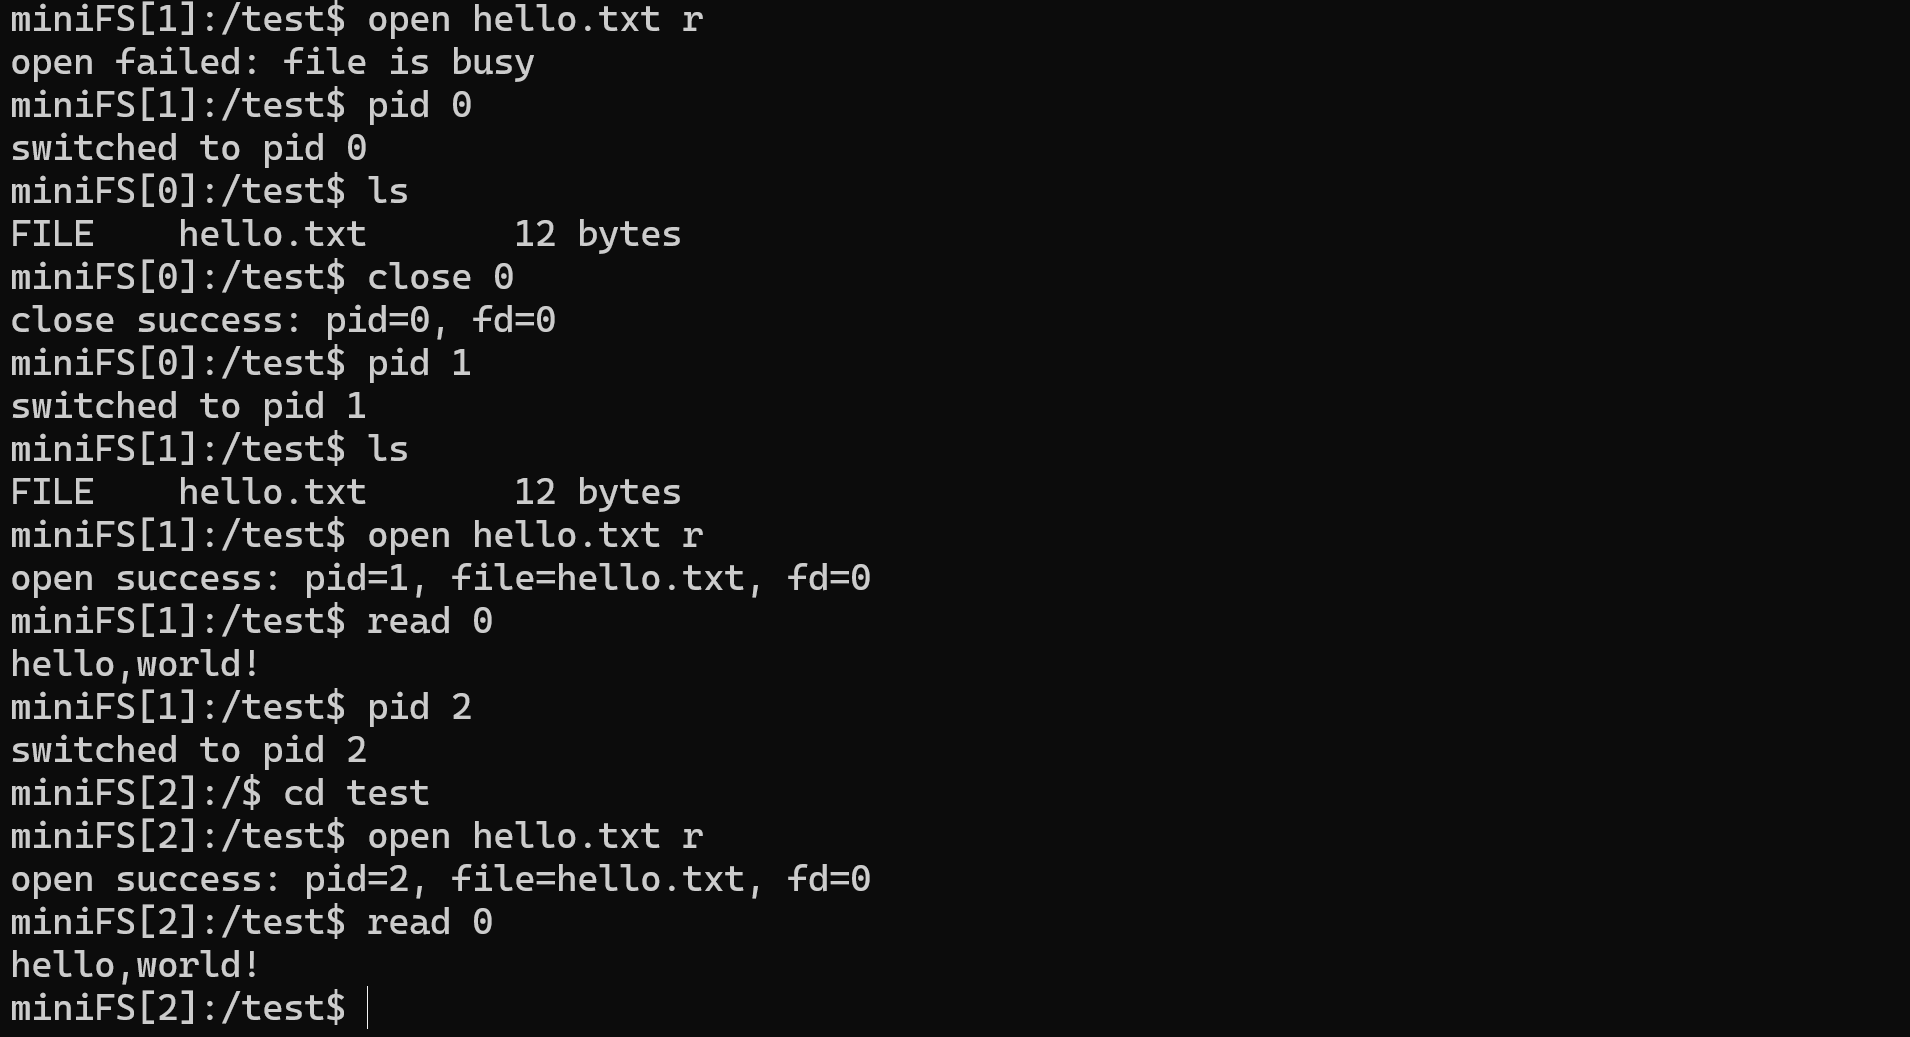
\includegraphics[width = 1\textwidth]{figure/task2_readerShare.png}
    \caption{读进程共享}
\end{figure}
如上图所示,多个读进程(pid=1,2)可以同时访问文件和目录,读取同一个文件的内容。

\begin{figure}[H]
    \centering
    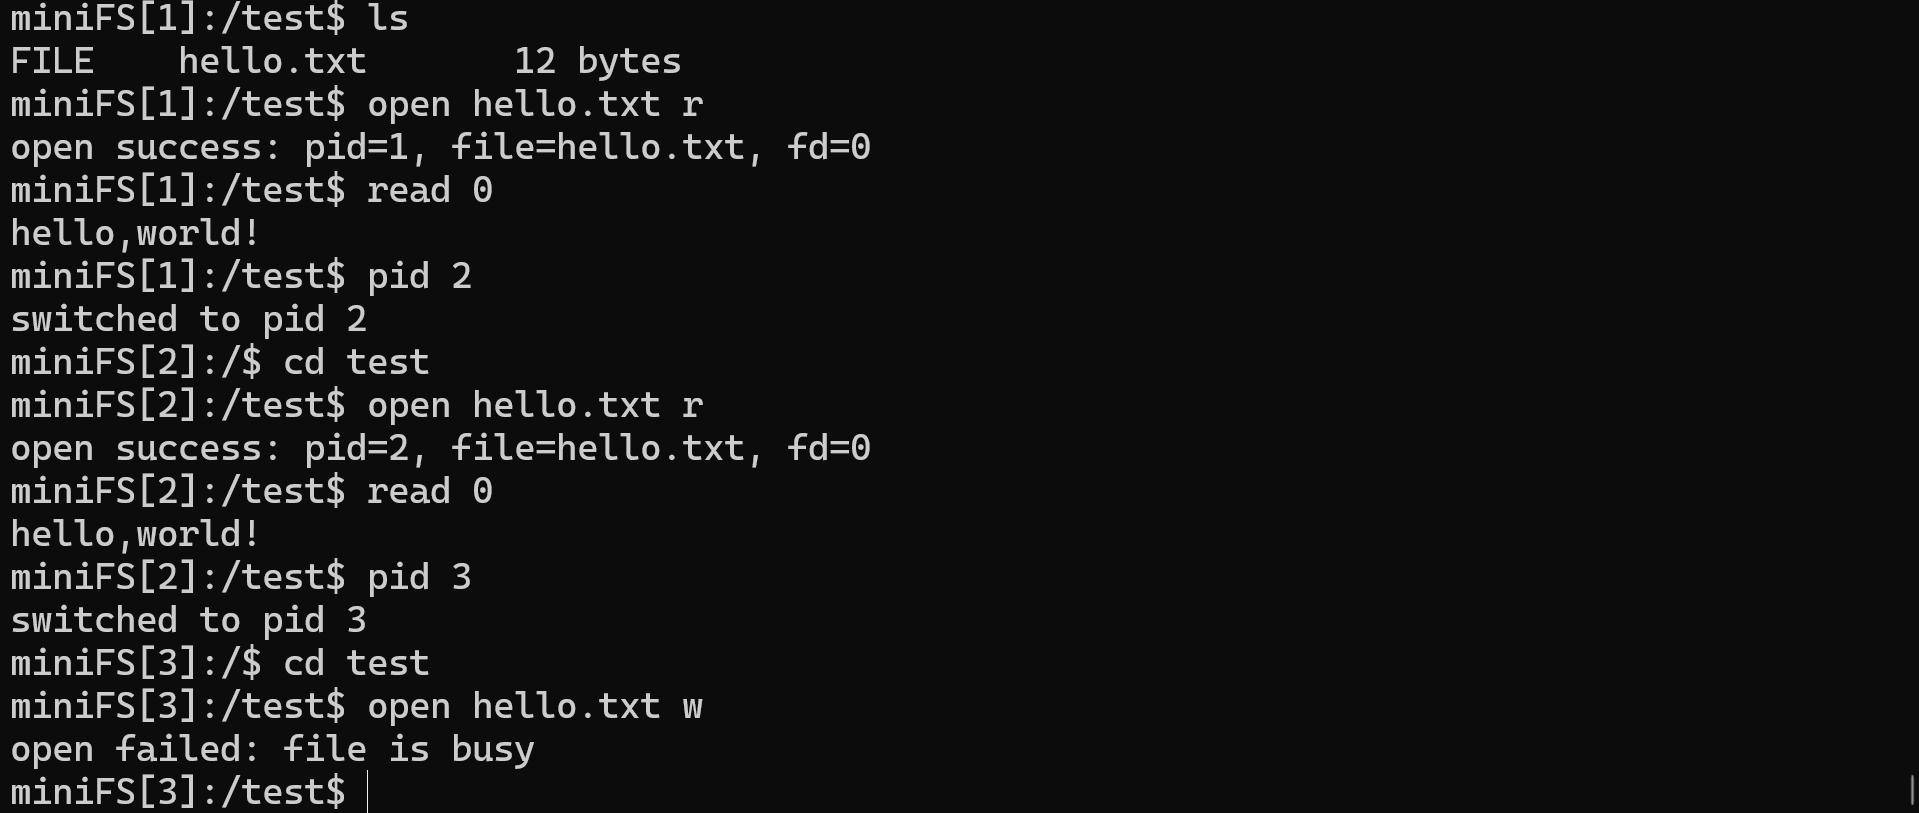
\includegraphics[width = 1\textwidth]{figure/task2_hasreader_writerFail.png}
    \caption{有读进程时写进程访问失败}
\end{figure}
如上图所示,当已经有读进程(pid=1,2)打开文件时,写进程(pid=3)无法访问文件,提示"file is busy",说明能实现读进程与写进程互斥访问文件的功能。
综上所述,该文件系统能够实现多进程之间的读者-写者互斥同步,读写操作均能正确执行,任务二成功完成。
